\chapter{Materialien}
\label{ch:materialien}

\section{Das \tit{Corpus der altdeutschen Originalurkunden}}
\label{sec:materialcao}

Das \tit{\citefield{frenz1998a}{maintitle}} definiert den Terminus
\term{Urkunde}\is{Urkunde} als \blockcquote[574]{frenz1998a}{schriftliche
Aufzeichnung über einen Vorgang rechtlicher Natur, die unter Beachtung gewisser
Formen geschieht und in einer bestimmten Weise beglaubigt ist; die
U\textins{rkunde} will eine rechtliche Wirkung erzielen und erhebt den Anspruch
der Glaubwürdigkeit.}

Diese Kriterien unterscheiden sie von anderen formal ähnlichen
Quellengattungen, wie zum Beispiel Akten oder Briefen. Nicht zu verwechseln mit
letzerem ist mittelhochdeutsch\il{Mittelhochdeutsch} \norm{brief}, mit dem
nicht nur Briefe, sondern auch Urkunden\is{Urkunde} bezeichnet werden, neben
\norm{hantvėste}
\autocites[][s.\,v.~\fw{brief}]{mwb1}[][s.\,v.~\fw{hantveste}]{mwb2}[vgl.
auch][]{schmidtwiegand1998a}.

Das \tit{Corpus der altdeutschen Originalurkunden} (\CAO) umfasst 4.617
Originalurkunden aus dem 13.\ Jahrhundert, das heißt keine zeitgenössischen
oder späteren Abschriften, von denen 4.289 deutschsprachig sind. Daneben
existieren in weitaus geringerem Maße Urkunden\is{Urkunde} auf
Mittelniederländisch\il{Mittelniederländisch} und Latein
\autocites[\RN{1}]{deboor1976}[25]{schulze2011}[40--41]{ganslmayer2012}.%
%
	\footnote{\citet[391]{gniffkerapp2005} geben die Gesamtzahl an
	Urkunden\is{Urkunde}, die das \CAO{} versammelt, mit 4.422 an. Die
	Diskrepanz in der Zählung ergibt sich dadurch, dass
	Parallelausfertigungen\is{Paralleltext} von ihnen nicht mitgezählt wurden
	\autocite[vgl.][40]{ganslmayer2012}.\label{fn:caowordcount}}
%
Beim Inhalt des \CAO{} handelt es sich nicht nur um Urkunden im engeren Sinn
\autocite[596]{schmidtwiegand1998b}. So sind gerade für die Frühzeit in der
ersten Hälfte des 13.~Jahrhunderts neben dem \tit{Erfurter Judeneid}
\autocites(Nr.~1, Erfurt, um 1200)[1,2--10]{cao1} und der \tit{Venusfahrt} aus
dem \tit{Frauendienst} Ulrichs von Liechtenstein\ia{Ulrich von Liechtenstein}
\autocites(Nr.~3, Schloss Liechtenstein, Bz.~Murtal, 1227)[5,13--40]{cao1}%
%
	\footnote{Vgl.\ München, Bayerische Staatsbibl., Cgm~44: 36va--37rb.
	% \autocite[1307]{hsc}.
	\citet[230--231]{schneider1987} datiert die Handschrift der Schrift nach
	auf \textquote{um 1300} und bestimmt ihren
	Schreibdialekt\is{Schreibdialekt} als niederösterreichisch\il{Bairisch}.}
%
auch diverse Stadtrechte enthalten, beispielsweise die von Braunschweig
\autocites(Nr.~2, 1227)[1,12--5,11]{cao1} und von Straßburg
\autocites(Nr.~N~238~A und B, 1283 bzw.\ Ende 13.~Jh.)[179,21--194.15;
179,29--194,32]{cao5}, sowie als ältester überlieferter deutschsprachiger
Rechtstext der \tit{Mainzer Reichslandfrieden} von 1235 in mehreren Fassungen
\autocites(Nr.~4)[14,11--17,55]{cao1}.%
%
	\footnote{Neben zwei lateinischen Fassungen (Nrn.~4~F und 4~Dor,
	\cite[5,42--9,17; 9,19--12,15]{cao1}) handelt es sich dabei um die
	folgenden Handschriften, die den Text auf deutsch in späteren Abschriften
	überliefern -- hier wurde eine Ausnahme vom Prinzip der \q{Originalurkunde}
	gemacht:
	%
	Nr.~4~D
		(\cite[14,11--15,53]{cao1};
		Dresden, Sächsische Landesbibl., Mscr.Dresd.M.32: 1r--v;
		Mitte 14.\ Jh.%
		% ; vgl.~\cite[7549]{hsc})
		),
	Nr.~4~P
		(\cite[12,17--14,09]{cao1};
		München, Bayerische Staatsbibl., Clm~16083: 2r;
		Mitte 13.\ Jh.; vgl.~\cites[256]{haas2010}%
		% [19293]{hsc}
		) sowie
	Nr.~4~W
		(\cite[14,11--17,55]{cao1};
		Wolfenbüttel, Herzog August Bibl., Cod.~Guelf.~3.1~Aug.~2º: 1r--3vb;
		3.~Viertel 14.~Jh.%
		% ; vgl.~\cite[8396]{hsc}
		).
	%
	Um frühe Originalurkunden im engeren Sinn handelt es sich bei den Nrn.~6--9
	und 39 \autocites[20,44--23,24;
	69,2--21]{cao1}[vgl.][15--16]{bertelsmeierkierst2008}.%
	}
%
Bei den meisten im \CAO{} enthaltenen Texten handelt es sich um
Privaturkunden\is{Urkunde}, insofern diese nicht von Kaisern oder Königen
ausgestellt wurden \autocites[vgl.][575]{frenz1998a}[585]{frenz1998b}. Einen
Eindruck von der enormen Variationsbreite der verhandelten -- vor allem sehr
alltagsnahen -- Gegen\-stände geben \citet[11]{schulze2011} und
\citet[35--36]{ganslmayer2012}. Auch die angesprochenen Themenfelder sind
vielfältig: \blockcquote[596]{schmidtwiegand1998b}{\textins{So} handelt es sich
im übrigen um Anweisungen, Verträge, Abmachungen, Geschäfte, Streitigkeiten und
deren Regulierungen seitens weltlicher und geistlicher Herren unterschiedlichen
Ranges, Institutionen wie Städten und Klöstern, Bürgern, Kaufleuten und
Handwerkern, freien und abhängigen Bauern, Mönchen, Nonnen und Kreuzfahrern.}

\begin{sloppypar}
Das \CAO{} ist ein Produkt jahrzehntelanger Sammeltätigkeit. Friedrich
Wilhelm\nocite{wilhelm1932} (1882--1939)%
% Quelle: https://d-nb.info/gnd/117380814
% Quelle: \autocite[2031]{bubenik2003}
, sein Begründer, verfolgte von Anfang an das Ziel, ein Textkorpus\is{Korpus}
bereitzustellen, das nicht durch \term{Normalisierung}\is{Normalisierung}, also
sprachliche Glättung und Vereinheitlichung
\autocites[vgl.][76--84]{bein2011}{kragl2015},
\blockcquote[\RN{60}]{wilhelm1932}{für den Sprachforscher unbrauchbar} gemacht
wurde. \posscite[161]{lachmann1820} ästhetischem Ideal von
\blockcquote[\RN{3}]{wilhelm1932}{jenem \q{unwandelbaren Hochdeutsch}, das
\q{die Dichter des dreizehnten Jahrhunderts bis auf wenig % \textins{sic}
mundartliche Einzelheiten \textelp{} redeten} \textelp{}, welches in seiner
sauberen Gleichmäßigkeit dem Latein klassisch-philo\-logi\-scher Schulausgaben
glich, und das \textelp{} nicht Eingeweihten ein Idealbild vorgaukelte} setzt
er konsequent und mit polemischer Schärfe sein Credo des möglichst
originalgetreuen Abdrucks entgegen.
\end{sloppypar}

In seinem \citetitle{deboor1976} zum abschließenden fünften Band des
\CAO{} hebt \citet[\RN{13}]{deboor1976} versöhnlich hervor, dass heute
niemand \blockquote{mehr bestreiten \textins{wird}, daß
die großen kritischen Ausgaben Karl Lachmanns\ia{Lachmann, Karl} und seiner
Nachfolger für die Forschung nötig und segensreich waren}, indem sie alte Texte
überhaupt wieder zugänglich und vermittelbar gemacht und damit
wissenschaftliches Interesse geweckt haben. Gegen die Frage der
\isi{Editionsphilologie} nach der Genese, \isi{Überlieferung} und
Rekonstruktion von Texten ist nichts einzuwenden.

Darüber hinaus sind normalisierte\is{Normalisierung} Formen auch aus
linguistischer Sicht nützlich, da sie sich unabhängig von individuellen Grafien
in unterschiedlichen Textzeugen als Zitations\-formen eignen. Moderne
technische Möglich\-keiten können die Anforderungen beider Parteien, der
Literaturwissenschaft\is{Editionsphilologie} und der historischen
Linguistik\is{Sprachgeschichte}, erfüllen, was das Spannungsfeld zwischen
Lesbarkeit, Textkritik und Datentreue betrifft, zumal auch die moderne
Editionstätigkeit radikales \q{Glattbügeln} von Texten, wie
\citet{wilhelm1932} es seinen Zeitgenossen vorwarf, durch das heute
größere Interesse an der Materialität der Textüberlieferung\is{Überlieferung}
eher scheut \autocite[vgl.][1306]{wegera2000}.%
%
	\footnote{Zum Beispiel stellt das Projekt \citetitle{ldmdigital} von
	\citet{ldmdigital} neben der diplomatischen Transkription\is{Transkription}
	mit dynamisch einblendbaren Abkürzungsauflösungen den
	normalisierten\is{Normalisierung} Editionstext\is{Editionsphilologie} der
	einzelnen Lieder zur Verfügung, sodass ein direkter Vergleich zwischen
	Handschrift, Transkription und Edition möglich ist, siehe
	\citeurl{ldmdigital}. Die in den vergangenen Jahren aufgebauten
	historischen Referenzkorpora des Deutschen (z.\,B.
	\cite[vgl.][522--523]{dipper2015}; \cite{rem}; \cite{ddd}) bieten neben
	diplomatischen Transkriptionen ebenfalls normalisierte Versionen der
	jeweiligen Textzeugen als Annotations-\is{Annotation} bzw.\
	Abstraktionsschicht.}

Dem Geist \citeauthor{wilhelm1932}s folgend betonen sowohl \citet{deboor1976}
als auch \citet{schulze2011} besonders den Wert des \CAO{} als
Korrektiv\is{Validierung} gegenüber den
mittelhochdeutschen\il{Mittelhochdeutsch} Grammatik\-darstel\-lungen wie zum
Beispiel der von \citet{paul2007}. So schreibt \citet[22]{schulze2011}, dass
zwar \textquote{\textins*{d}ie Vorbehalte\is{Vorbehalt} gegenüber der
Urkundenauswertung\is{Urkunde} \textelp{} inzwischen weitgehend geschwunden}
seien. Zum damaligen Zeitpunkt waren aber nach wie vor
\blockcquote[22]{schulze2011}{\textins*{w}ichtige Aspekte zur
mittelhochdeutschen\il{Mittelhochdeutsch} Grammatik \textelp{} nicht primär auf
sprachgeografische\is{Dialektgeografie} Zuordnungen ausgerichtet. Bei
syntaktischen Untersuchungen verschiedener Art gibt es viele übergreifende
Fragen und Beobachtungen, für die das besondere Quellenmaterial ergiebig ist
und die allenfalls zusätzlich sprachgeographisch\is{Dialektgeografie} weiter
differenziert werden können.}

Auch \citet{wegera2000} bemerkt kritisch, dass in den Grammatiken des
Mittelhochdeutschen\il{Mittelhochdeutsch} nach Paul\nocite{paul2007} und
\citeauthor{mettke1993} \blockcquote[1305]{wegera2000}{\textins*{k}eine der
Textsammlungen adäquat die regionale Variabilität oder die \isi{Diachronie} von
drei Jahrhunderten wider\textins*{spiegelt}, noch \textelp{} eine
Textsortenspezifik sichtbar \textins*{wird}. Den Schwerpunkt bilden in allen
Fällen die poetischen Denkmäler des späten 12.\ und frühen 13.~Jhs.\ obd.\
Provenienz. Einige wenige Urkunden\is{Urkunde} und andere Prosatexte\is{Prosa}
\textelp{} werden zwar genannt, doch bei der Auswertung kaum berücksichtigt.}

Das Textkorpus\is{Korpus} zur neuen
\tit{Mittelhochdeutschen\il{Mittelhochdeutsch} Grammatik} \autocite{ksw3,ksw2}
versucht hier gegenzusteuern durch ein bezüglich Zeit, Sprachräumen und
Textsorten sorgfältig ausbalanciertes Textkorpus, das auf repräsentativen
Exzerpten möglichst von Original\-handschriften basiert
\autocites[1311--1318]{wegera2000}[3]{kleindipper2016}. Auch
Urkunden\is{Urkunde} sind Teil dieses Korpus, doch nur zu einem relativ
geringen Teil. In den 103 gelisteten Quellen des Grammatik-Korpus \autocite%
	% [19--30]{ksw3}%
	[14--26]{ksw2} sind die zehn in \tabref{tab:kswurk} aufgeführten
Urkundenstrecken mit insgesamt 225 Urkunden enthalten. Dabei werden für das
13.~Jahrhundert das Hessische\il{Hessisch}, Rheinfränkische\il{Rheinfränkisch},
Ostmitteldeutsche\il{Ostmitteldeutsch}, Bairische\il{Bairisch} und
Ostfränkische\il{Ostfränkisch} aufgrund der Aufnahmebedingungen nicht abgedeckt
\autocite[vgl.][1311]{wegera2000}. Da auch für die abgedeckten Dialektregionen
Mittelfränkisch\il{Mittelfränkisch}, Alemannisch\il{Alemannisch} und
Schwäbisch\il{Schwäbisch} jeweils nur eine große Stadt als Schreibzentrum
aufgenommen wurde, ist kritisch zu fragen, ob die Auswahl für das
13.~Jahrhundert tatsächlich repräsentativ ist.%
%
	\footnote{Die einzelnen enthaltenen Texte können
	\citet[Textübersicht]{kleindipper2016} entnommen werden. Laut dieser Liste
	sind aus dem \CAO{} enthalten: Nrn.~53, 60, 61, 71, 72~A, 72~B, 74, 75, 76,
	78, 79, 83, 85, 223, 224, 428, 429, 508, 548~A, 548~C, 549, 560, 658, 677,
	780, 831, 1371, 1542, 1639, 1648, 1651~B, 1678, 1686, 1768, 1883, 1958,
	1959, 1985, 2001, 2008, 2112, 2133, 2182, 2277, 2348, 2461, 2643, 2681,
	2725, 2733, 2767, 2780, 2861, 2909, 2921, 2936, 3018, N~36, N~68, N~163,
	N~272.\label{fn:kswcao}}

\begin{table}
\centering
\caption{Urkundenstrecken im Korpus zu \citet{ksw3,ksw2}}
\begin{tabular}{l l l r}
\lsptoprule
Zeit & Ort & Schreibdialekt & \makecell[r]{Anzahl\\ Urkunden}\\\midrule

2.~Hälfte 13.~Jh.
	& Köln
	& mittelfränkisch
	& 18
	\\

%
	& Freiburg i.~Br.
	& alemannisch
	& 35
	\\

%
	& Augsburg
	& schwäbisch
	& 9
	\\

\cmidrule{2-4}

%
	& Summe
	& \mc{2}{r}{62}
	\\

\midrule

1.~Hälfte 14.~Jh.
	& Köln
	& mittelfränkisch
	& 15
	\\

%
	& Mainz
	& rheinfränkisch
	& 30
	\\

%
	& Jena-Weida
	& ostmitteldeutsch
	& 7
	\\

%
	& Freiburg i.~Br.
	& alemannisch
	& 29
	\\

%
	& Nürnberg
	& ostfränkisch
	& 37
	\\

%
	& Augsburg
	& schwäbisch
	& 21
	\\

%
	& Landshut
	& bairisch
	& 24
	\\

\cmidrule{2-4}

%
	& Summe
	& \mc{2}{r}{163}
	\\

\midrule

Gesamt
	& \mc{3}{r}{225}
	\\

\lspbottomrule
\end{tabular}
\label{tab:kswurk}
\end{table}

Wenn \citeauthor{schulze2011} bemerkt, dass in jüngerer Zeit
Vorbehalte\is{Vorbehalt} gegenüber Urkunden\is{Urkunde} als sprachhistorischer
Quelle zurückgegangen sind, spielt sie dabei wohl auf das von
\citet[23--33]{boesch1946} und \citet[389]{haacke1955} geäußerte, für
grundlegend gehaltene Erfordernis der
Schrei\-ber\-identifizierung\is{Schreiberidentifizierung} an, das sich lange
Zeit stark hemmend auf die Erforschung des \CAO{} ausgewirkt hat
\autocite[21--22]{schulze2011}. Misstrauen in der älteren Forschung gegenüber
einzelnen Urkunden\-texten, vor allem solchen mit unbekanntem Schreiber,
gründet sich auf die Beobachtung, dass der bezeichnete oder indirekt ermittelte
Ausstellungsort nicht zwingend der Herkunftsort des Schreibers sein muss
\autocite[16]{schulze2011}, wodurch zumindest die Möglichkeit der Diskrepanz
zwischen dessen gesprochenem Dialekt und dem \isi{Schreibdialekt} des
Urkundentexts besteht.

Auch wenn also nicht gewährleistet werden kann, dass sich der Herkunftsort des
Schreibers\is{Schreiberidentifizierung}, der Schreibort der jeweiligen
\isi{Urkunde} und ihr Ausstellungsort gleichen,
\blockcquote[331--332]{ganslmayeretal2003}{nimmt \textins{der Ausstellungsort}
aber in jedem Fall in irgendeiner Weise Bezug zu dem geschehenen Rechtsakt
\textelp{}. Deshalb kann insgesamt davon ausgegangen werden, dass durch den
Ausstellungsort der geographische\is{Dialektgeografie} Entstehungsraum der
Urkunde erfassbar ist}. Darüber hinaus gilt, \blockcquote[122]{deboor1974}{daß
die einzelne Urkunde für eine sprachliche Untersuchung nur einen sehr bedingten
Aussagewert hat. Erst die Belegmengen schaffen die feste Grundlage gesicherter
Erkenntnisse und gestatten es, Einzelgänger als solche zu erkennen und
auszusondern.}

Ein weiteres Misstrauensargument\is{Vorbehalt} ist die von
\citet[1311]{wegera2000} angesprochene \blockquote{sich wiederholende
\isi{Formelhaftigkeit}}. Damit verwandt ist auch die Annahme,
Urkunden\is{Urkunde} würden aufgrund ihrer Rechtsthematik eine besondere
juristische \isi{Fachsprache} verwenden. Zwar ist nicht zu leugnen, dass
bestimmte Teile des Formulars in gleicher oder ähnlicher Formulierung oder
bestimmte formelhafte Wendungen (vgl. \sectref{phsec:formelhaftigkeit}) immer
wiederkehren, wie zum Beispiel Publikationsformeln ähnlich \norm{Ich tue kunt
allen dęn die disen brief sęhent oder hȫrent lęsen} \wdef{Ich mache bekannt
allen denen, die diese Urkunde sehen oder lesen hören} oder auch die
obligatorischen Beglaubigungs- und Datierungsformeln.%
%
	\footnote{% 
	% Für weitere Beispiele siehe \citet[10, Fußnote 5--8]{schulze2011}.
	Trotz ihrer \isi{Formelhaftigkeit} lassen sich diese Teile aufgrund ihrer
	breiten \isi{Überlieferung} als \isi{Paralleltext} verwenden
	\autocite[siehe][]{cysouwwaelchli2007}. Beispielhafte, das \CAO{}
	betreffende Überlegungen dazu stellen
	\citet[174--175]{beckerschallert2022b} an.}

\citet[13, 25--38]{schulze2011} weist jedoch nach, dass die Dispositio, die den
Inhalt der mündlich\is{Mündlichkeit} geführten Verhandlung wiedergibt, frei und
vor allem ohne Umweg über das Lateinische\il{Lateinisch}\is{Latinität}
formuliert ist, obgleich integrale Bestandteile des
Urkundenformulars\is{Urkunde} aus der lateinischen\il{Lateinisch}
Urkundentradition übernommen wurden. Sie attestiert den Urkunden des \CAO{}
\blockcquote[3]{schulze1994}{einen selbständigen Wort- und Formelschatz und
eine eigene Syntax \textelp{}. \textins{Die Urkunden} geben ein vielfältiges
Bild einer variantenreichen, geschriebenen
Gebrauchs\-sprache\is{Gebrauchssprache}}.

Zuletzt bleibt noch etwas zu editorischen Eingriffen\is{Normalisierung}
insbesondere ab Band~4\nocite{cao4} zu sagen. Bei der vorliegenden Studie ist
bezüglich der Treue der \isi{Transkription} von Belang, dass die Schreibung
solcher Laute, deren Schriftwiedergabe auf \norm{u} basiert (das heißt \norm{u,
ū, ü, ǖ, iu, ue} und \norm{üe}), besonders großer Variabilität unterliegt.
Wenn also auch die Möglichkeit besteht, dass ein Diakritikum über einem \lit{u}
oder \lit{v} nicht hundertprozentig der Form der Handschrift entspricht, ist
nicht damit zu rechnen, dass die Interpretation des Graphems dadurch
grundsätzlich fehlgeleitet würde. Abgesehen von % Hyperkorrekturen und möglichen
Flüchtigkeitsfehlern in Transkription und Druck, die selbst \citet[\RN{60},
\RN{78}]{wilhelm1932} nicht ausschließt, ist gemäß den
Editionsgrundsätzen\is{Editionsphilologie} des \CAO{} nicht damit zu rechnen,
dass ein vermeintlich unregelmäßiges \lit{-iu} zu \norm{-e} emendiert wurde und
umgekehrt. Auch hier gilt der Grundsatz, dass nur die Menge der Urkunden ein
repräsentatives Bild abgibt.

Ein gewichtiger Vorteil des \CAO{} ist, dass Urkunden\is{Urkunde} in vielen
Fällen nicht nur datiert sind, sondern sie sich entweder direkt durch die
Nennung des Ausstellungsorts oder indirekt über Ortsangaben und beteiligte
Personen auch geografisch\is{Dialektgeografie} lokalisieren lassen
\autocite[16]{schulze2011}.%
%
	\footnote{\citet[393]{gniffkerapp2005} geben an, dass
	\blockquote{\textins*{i}n fast 60 Prozent der Urkunden\is{Urkunde}
	\textelp{} der Schreibort und/oder die Urkundspartei (Aussteller/Empfänger)
	genannt \textins{werden}, was eine erste Lokalisierung ermöglicht}. Die
	Online-Edition des \CAO{} \autocite{cao-online}, deren Daten hier zur
	Auswertung verwendet wurden, enthält gegenüber den gedruckten Bänden
	Ergänzungen, Korrekturen und Nachträge
	\autocite[vgl.][393--394]{gniffkerapp2005}.}
%
Das Material hat eine Schlagseite in Richtung des
Westoberdeutschen\il{Westoberdeutsch}, und hier besonders zum
Oberrheinischen\il{Alemannisch} und Hochalemannischen\il{Alemannisch} hin, da
die volkssprachige\is{Volkssprache} Beurkundung in diesem
Sprachraum\is{Dialektgeografie} früher als im ostoberdeutschen\il{Bairisch}
eingesetzt hat \autocites[1774]{skala1985}[15]{schulze2011}.

Einen Überblick über die geografische Verteilung\is{Distribution!geografische}
der Belegorte und zuordenbaren Urkunden\is{Urkunde} gibt
\figref{fig:cao_urkorte}. Die Karte stellt die deutschen\il{Neuhochdeutsch}
Dialektlandschaften auf dem Stand des frühen 20.~Jahrhunderts dar, inklusive
der Gebiete außerhalb der modernen Grenzen Deutschlands, Österreichs,
Liechtensteins und der Schweiz, in denen zu dieser Zeit aufgrund der
politischen Situation auch Deutsch\il{Neuhochdeutsch} gesprochen wurde.%
%
	\footnote{Verzerrungen in der Beschriftung der Karte und im Kartenbild
		selbst sind ein Artefakt der Reprojektion ins WGS-84-Format bei der
		Verarbeitung mit \citetitle{qgis} \autocite{qgis}.}
%
Eine vergleichbare Darstellung der mittelhochdeutschen\il{Mittelhochdeutsch}
Dialekträume basierend auf historischen\is{Diachronie} Quellen selbst, ohne
Rückprojektion der neuzeitlichen Situation, ist mir nicht bekannt. Unter dem
von \citet[4]{paul2007} geäußerten \isi{Vorbehalt}, dass \textquote{die
modernen Sprachraumkonturen\is{Dialektgeografie} keinesfalls vorschnell und
unkritisch auf die mittelhochdeutsche\il{Mittelhochdeutsch} Zeit übertragen
werden \textins{dürfen}}, soll die Karte hier zur groben Orientierung dienen.

\begin{figure}
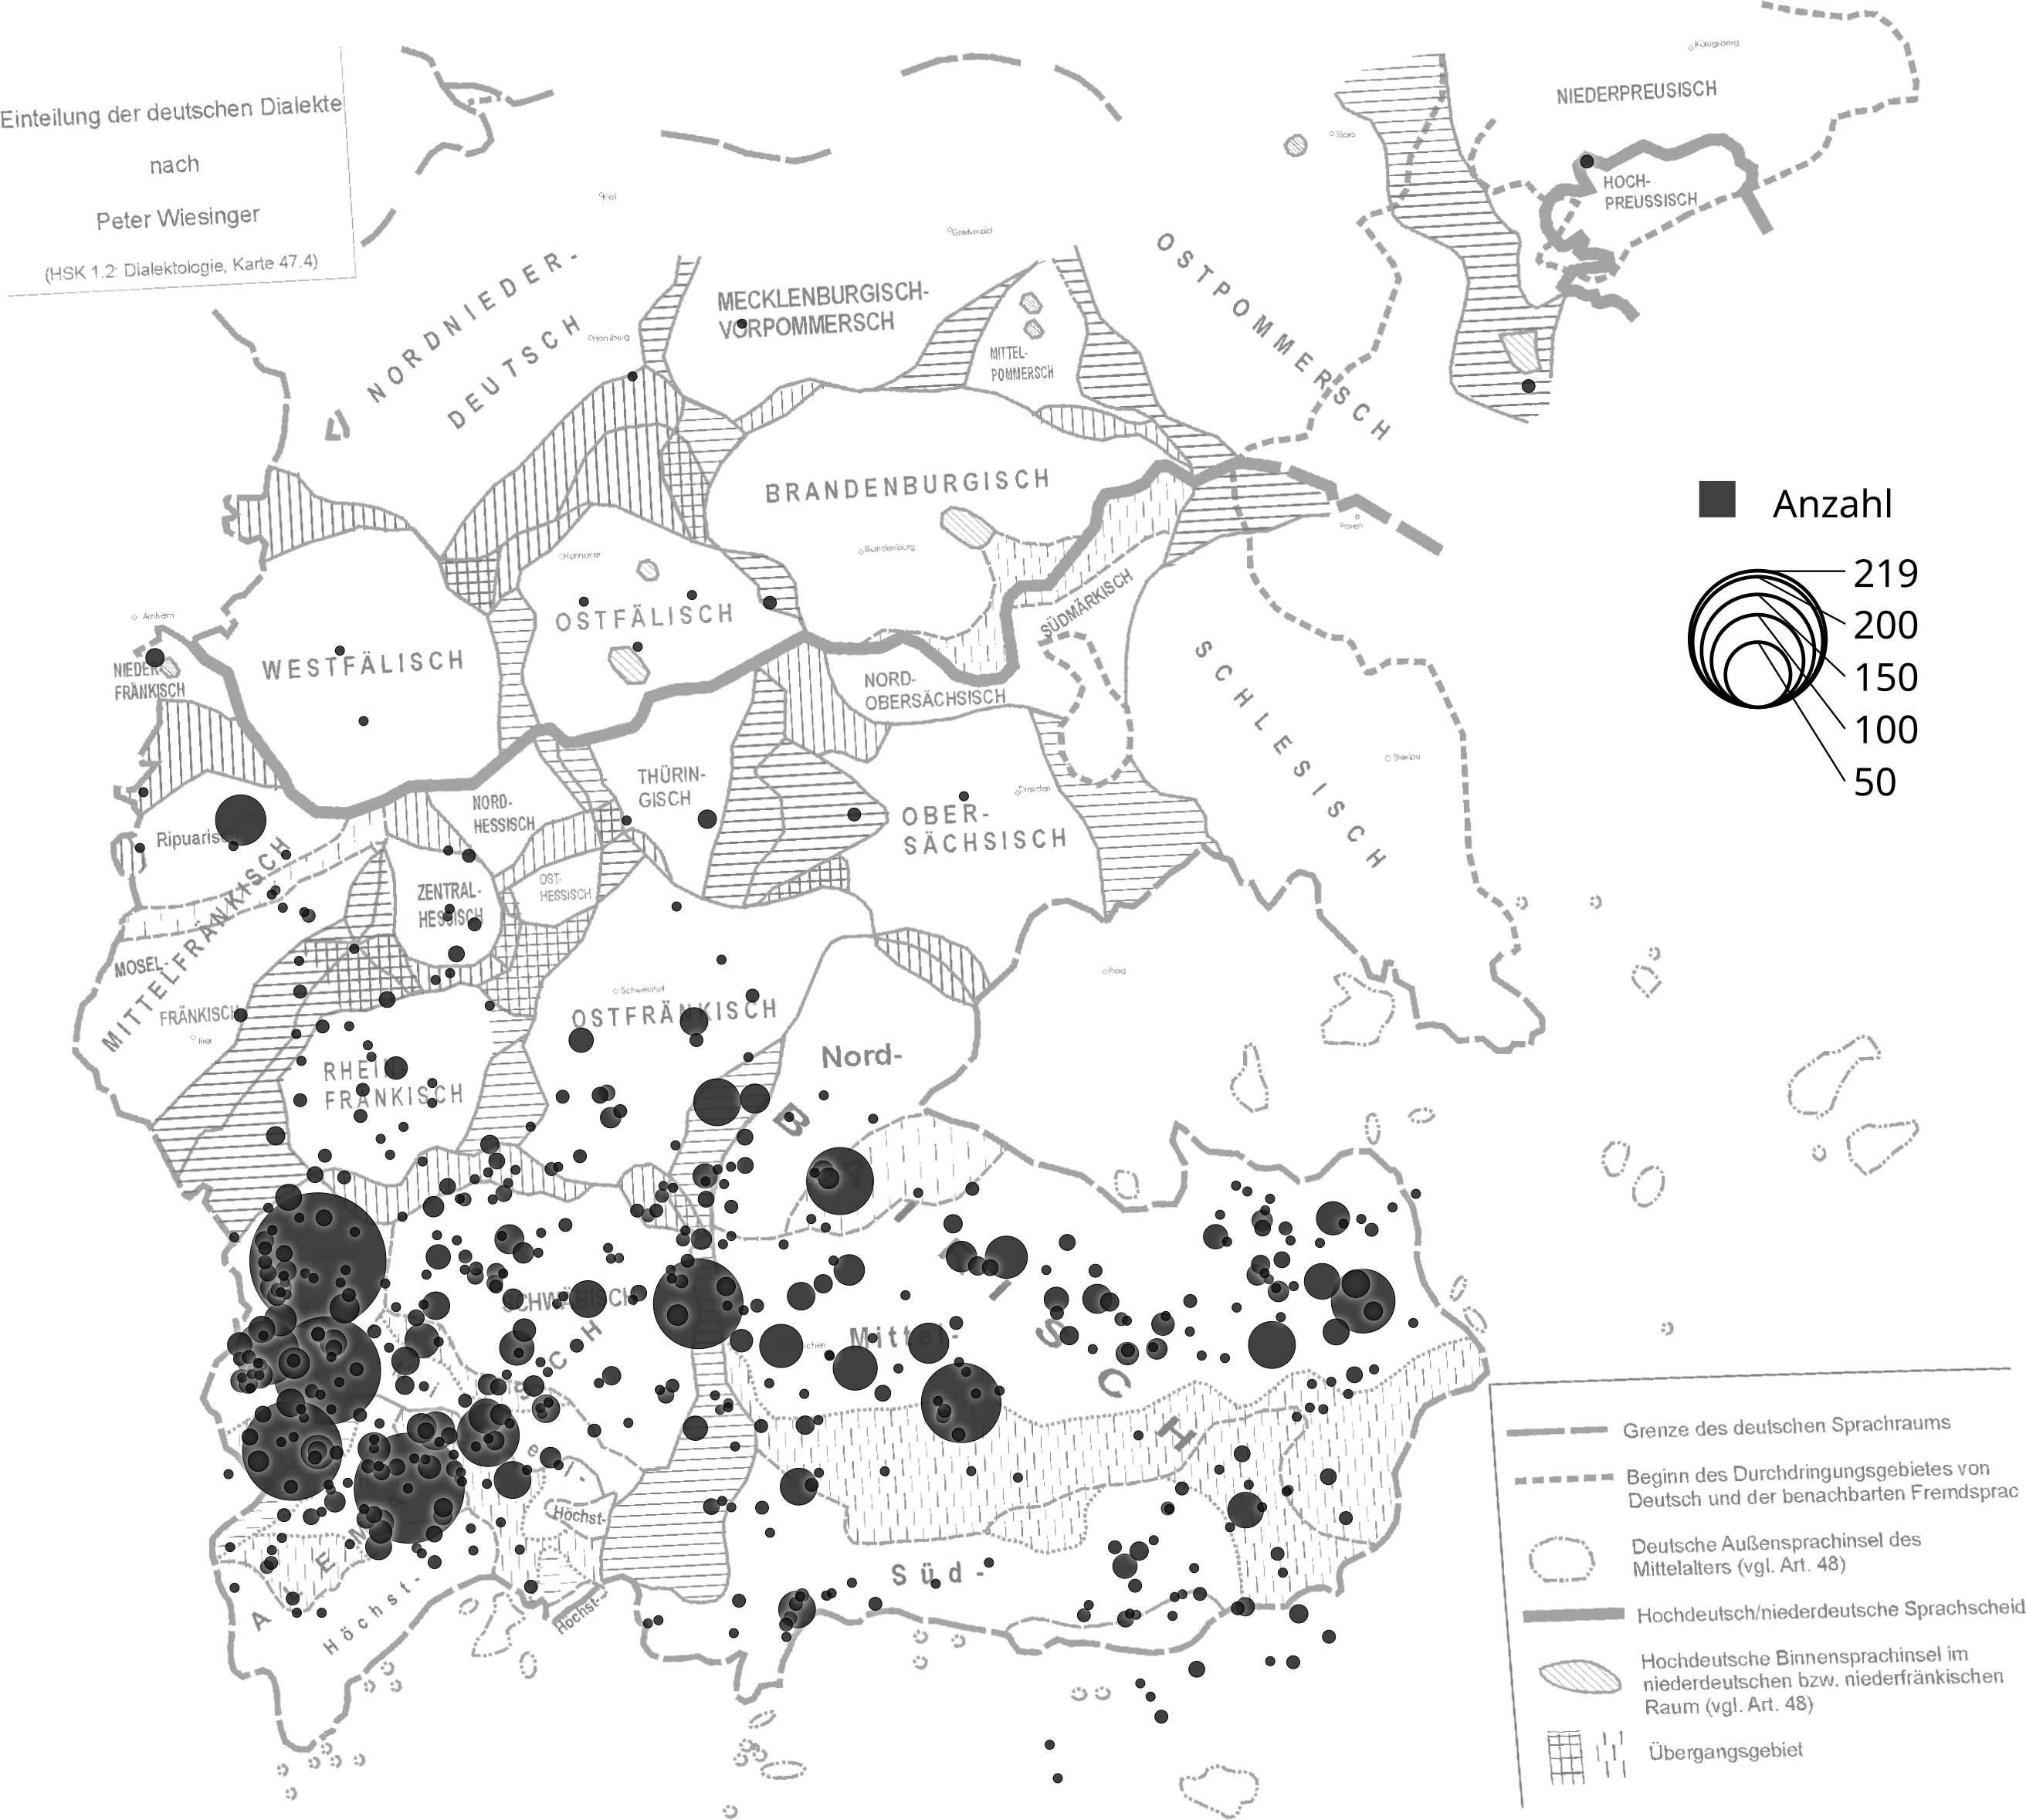
\includegraphics[
	width=\linewidth,
	keepaspectratio
]{./figures/2022-03-03_deedsperplace.png}
\caption{Urkunden pro eindeutigem \CAO{}-Ausstellungsort
	(Hintergrundkarte: \cite{wiesinger1983:rede})
}
\label{fig:cao_urkorte}
\end{figure}

Das \CAO{} hat den Anspruch, die gesamte
Urkundenüberlieferung\is{Überlieferung}\is{Urkunde} des 13.~Jahrhunderts zu
versammeln. Auch wenn es eine \q{Dunkelziffer} an Urkunden gibt, die nicht in
die Sammlung aufgenommen wurden, wird die Zunahme an deutschsprachigen Urkunden
in \tabref{tab:urkstat} deutlich; der Großteil der Urkunden im \CAO{} entfällt
auf die letzten beiden Jahrzehnte. Während der
westoberdeutsche\il{Westoberdeutsch} Sprachraum\is{Dialektgeografie} zunächst
bei der Ausstellung deutschsprachiger Urkunden führt, holt der
ostoberdeutsche\il{Bairisch} ab den 1280er Jahren massiv auf und übertrifft den
westoberdeutschen\il{Westoberdeutsch} am Ende der Dekade schließlich um etwa
4,6\,\% \autocite[46--47]{ganslmayer2012}.%
%
	\footnote{\citet[47]{ganslmayer2012} weist im Abschnitt von 1290--1299 für
		das Alemannisch\il{Alemannisch}-Schwäbische\il{Schwäbisch} 38,79\,\%
		der im \CAO{} enthaltenen Urkunden aus sowie für das
		Bairische\il{Bairisch} insgesamt 43,4\,\%. }

\begin{table}
\centering
\caption{Anzahl der Urkunden im \tit{Corpus der altdeutschen Originalurkunden}
pro Jahrzehnt \autocite[40]{ganslmayer2012}}
\begin{tabularx}{\textwidth}{l C C C C}
\lsptoprule
%
	& {bis 1279}
	& {1280--89}
	& {1290--99}
	& {Summe}\\

\midrule

Anzahl insgesamt
	& 621
	& 1.095
	& 2.901
	& 4.617
	\\

davon deutschsprachig
	& 585
	& 1.007
	& 2.697
	& 4.289
	\\

\lspbottomrule
\end{tabularx}
\label{tab:urkstat}
\end{table}

Insgesamt lässt sich festhalten, dass die Urkunden\is{Urkunde} des \CAO{} für
linguistische Fragestellungen eine Reihe von Vorteilen bieten. Zum einen
handelt es sich um Gebrauchsprosa\is{Prosa}\is{Gebrauchssprache}, die im Rahmen
von großteils privaten Rechtsgeschäften das alltägliche Leben der Zeit in
vielfältiger Weise berühren. Damit stehen die Urkundentexte tendenziell näher
an der Alltagssprache als literarische Texte, die besonders in der älteren
Grammatikschreibung zum Mittelhochdeutschen überproportional repräsentiert
waren\is{Korpus}. Die Urkunden stellen in der Regel das schriftlich
festgehaltene Ergebnis mündlich\is{Mündlichkeit} geführter Verhandlungen dar
\autocite[595]{schmidtwiegand1998b}. Zum anderen ist das \CAO{} für
sprachgeschichtliche\is{Sprachgeschichte} Untersuchungen gut geeignet, da
größter Wert auf eine zuverlässige \isi{Transkription} gelegt wurde. Die
Urkunden sind darüber hinaus zumeist datiert und enthalten Informationen, mit
denen sie sich regional zuordnen lassen, was gerade für
sprachgeografisch\is{Dialektgeografie} orientierte Analysen eine ideale
Voraussetzung ist \autocite[22]{schulze2011}.

Obwohl bei der vorliegenen Untersuchung nicht sämtliche Urkunden\is{Urkunde}
untersucht wurden (vgl. \sectref{sec:miningcao}), ist das Ortsnetz dicht genug,
dass Raumstrukturen\is{Dialektgeografie} zutage treten. Besonders hervorzuheben
ist der Umstand, dass das insgesamt zirka zwei Millionen Wortformen umfassende
Textkorpus\is{Korpus} (das heißt einschließlich der Mehrfachausfertigungen und
nicht-deutschsprachiger Urkunden) vollständig elektronisch vorliegt
\autocites{gniffkerapp2005}{cao-online} und damit eine ansehnliche Datenmenge
in ihrer ganzen Breite handhabbar wird
\autocite{beckerschallert2021,beckerschallert2022b}.%
%
	\footnote{Zum Vergleich mit anderen elektronischen Korpora zu
	historischen\is{Diachronie} Sprachstufen des Deutschen siehe
	\citet{dipper2015}. \citet[391]{gniffkerapp2005} beziffern den Umfang des
	\CAO{} mit \blockquote{etwa 1,3 Millionen Belegwörtern}, wobei sie sich
	dabei vermutlich nur auf das deutschsprachige Material ohne
	Doppelausfertigungen beziehen.} % (vgl.~\sectref{fn:caowordcount}).}

Nachteilig ist, dass nicht an jedem Ort gleich große Mengen an
Urkunden\is{Urkunde} vorliegen, zumal die Urkunden des \CAO{} lediglich eine
Momentaufnahme größtenteils der letzten zwanzig Jahre des 13.~Jahrhunderts
bieten. Darüber hinaus besteht das Problem, dass sich Schreiberinnen und
Schreiber in der Regel nicht greifen lassen\is{Schreiberidentifizierung}, sodass
aus der einzelnen Urkunde heraus nicht deutlich wird, ob sie genuin
ortstypische Sprache reflektiert. Diesen Nachteilen lässt sich jedoch mit einer
Kombination von quantitativer und qualitativer Analyse begegnen. Da einzelne
Belege wenig aussagen, braucht es eine gewisse Masse an Belegen, um Tendenzen
deutlich zu machen\is{Validierung}. Zu kleinteiligen Aus\-sagen zur Mundart
einzelner Orte wird man über die Untersuchung der Urkunden nicht gelangen, wohl
aber zu Aussagen über das Verhalten unterschiedlicher Schreibregionen und die
Reflexion divergierender Sprachmerkmale im regionalen Schreibgebrauch.

%%%%%%%%%%%%%%%%%%%%%%%%%%%%%%%%%%%%%%%%%%%%%%%%%%%%%%%%%%%%%%%%%%%%%%%%%%%%%%%

\section{Die \tit{Kaiserchronik}}
\label{sec:materialkc}

Die \tit{Kaiserchronik} (\KC{}) ist eine \isi{Reimchronik} in deutscher
Sprache, die um die Mitte des 12.~Jahrhunderts vermutlich in Regensburg
entstanden ist.%
%
	\footnote{Einen Überblick bietet \citet{nellmann1983}. Zum aktuellen
		Forschungs- und Editionsstand\is{Editionsphilologie} siehe
		\citet{chincaetal2019a} sowie jüngst die Dissertation von
		\citet{weis2022}. Angaben zur Entstehungszeit und zum
		\isi{Schreibdialekt} der jeweiligen Textzeugen basieren auf dem derzeit
		noch unveröffentlichten Katalog von \citet{wolf:kckat}, siehe auch
		\citeurl{kcdigital}\nocite{kcdigital} sowie
		\citet[s.\,v.~\tit{Kaiserchronik}]{hsc} mit den dort angegebenen
		Quellen.}
%
Sie ist anonym überliefert und auch die Frage nach ihrem Auftraggeber ist
ungeklärt. \citet[92]{wolf2008} bescheinigt der \KC{}
\blockquote{ein Formen-, Sprach- und Normeninventar, das für die
volks\-sprachig-höfische Literatur des Spätmittelalters zu einem Grundmuster
wird}.

Der Text ist in bislang fünfzig bekannten Textzeugen zwischen dem letzten
Viertel des 12.~Jahrhunderts (A1) und dem späten 16.~Jahrhundert (T)
überliefert \autocite[39, 57]{wolf:kckat}; der
Überlieferungsschwerpunkt\is{Überlieferung} fällt in das 13.~Jahrhundert
\autocites[vgl.][s.\,v.~\tit{Kaiserchronik}]{hsc}{kcdigital}. Im Lauf ihrer
etwa vierhundertjährigen Überlieferungsgeschichte hat die \KC{} zwei
Überarbeitungen erfahren: um ca.~1200 (Rezension~B) und um ca.~1250
(Rezension~C) \autocites{wolf2008}. \citet[369]{gaertner1995} zufolge
unterscheiden sich die Rezensionen B und C so stark von der ältesten Fassung
(Rezension~A), dass sie jeweils neue Werke darstellen;
\citet[142]{chincaetal2019a} sprechen mit \citet{bumkepeters2005} in diesem
Zusammenhang von \q{\isi{Retextualisierung}}.

Die \KC{} handelt ihrer eigenen Aussage nach \norm{von den bâbesen unt von den
chu\-nigen, baidiu guoten unt ubelen} \wdef{von den Päpsten und von den
Königen, sowohl guten als auch schlechten} (\KC: V.~19--20;
\cite[79]{schroeder1895}). Die einzelnen Episoden zu den jeweiligen Kaisern von
Cäsar bis Konrad~III.\ (A/B), beziehungsweise je nach Fortsetzung Friedrich~II.
oder Rudolf~I. (C), verselbstständigen sich bisweilen zu eigenen Erzählungen
und haben eher den Charakter eines Fürstenspiegels\is{Fürstenspiegel} als den
eines strikt historiografischen Abrisses, zumal die historische Reihenfolge der
Kaiser nicht immer eingehalten wird, zwei römische Kaiser hinzugedichtet werden
und die Angaben zu den Regierungszeiten der jeweiligen Kaiser am Ende jeder
Episode willkürlich sind \autocite[954--960]{nellmann1983}. Stattdessen soll
\blockcquote[957]{nellmann1983}{\textins*{m}öglichst jede Kaisergeschichte
\textelp{} den \textquote{heilsgeschichtlichen Kampf der guten und der bösen
Mächte} \textelp{} zur Anschauung bringen}.

Erste Ausgaben des Volltexts der \KC{} erfolgten von \citet{massmann:kukb}
sowie von \citet{diemer1849} nach der damals gerade neu entdeckten Vorauer
Handschrift (A1). Die bisher maßgebliche Edition ist die von
\citet{schroeder1895}. Die genannten drei Editionen geben alle den Text
der Rezension~A wieder, \citeauthor{massmann:kukb} bietet ausschnittsweise auch
Teile von B und C.%
%
	\footnote{Ein kritisches Resümee zu \citeauthor{massmann:kukb}s
		Editionstätigkeit\is{Editionsphilologie} zieht \citet{wolf2023}, in
		Bezug auf die \KC{} siehe dort, \notecite[\pno~122--132]{wolf2023}.
		\citeauthor{massmann:kukb}s Edition der \KC{} beruht auf der
		Heidelberger A-Handschrift (H), deren Text er mäßig normalisiert im
		Grunde als \isi{Leithandschrift} bietet, allerdings ermangelt sein Text
		bisweilen philologischer Stringenz und ist damit nicht unproblematisch
		\autocite[125--126]{wolf2023}. Obwohl \citeauthor{massmann:kukb} nach
		\posscite[131--132]{wolf2023} Urteil zugute zu halten ist, dass in den
		\textquote{Beigabenpaketen} auch zur \KC{}-Edition durchaus viel
		Nützliches an Meta-, Inter- und Paralleltexten\is{Paralleltext}
		enthalten ist, zeichnen sich diese Beigaben durch \textquote{eine
		überbordende Fülle gepaart mit einer chaotisch anmutenden Un-Ordnung}
		negativ aus, \textcquote[131]{wolf2023}{und zwar insbesondere dann,
		wenn Fakten und Phantasie (bei Maßmann nicht selten) zusammenfließen},
		vor allem im Sinne seiner vom Nationalismus geprägten
		politisch-historischen Interessen.%
	}
%
Die Edition von \citeauthor{schroeder1895} ist zwar insofern normalisiert, als
Schreibweisen vereinheitlicht sowie Vokal\-längen und moderne Interpunktion
eingefügt wurden. Sie verfolgt im Großen und Ganzen aber das
Leit\-handschriften\-prinzip\is{Leithandschrift} auf der Grundlage von A1.
\citeauthor{diemer1849} stellt einen diplomatischen Abdruck zur Verfügung. Eine
textkritische Ausgabe,\is{Editionsphilologie} die die Texte der Rezensionen~B
und C als gleichberechtigt neben A behandelt, ist bisher ein \isi{Desiderat}.

Mit dem Projekt zur Neuedition\is{Editionsphilologie} der \KC{} in Form einer
synoptischen Ausgabe wird die Einlösung dieses Desiderats\is{Desiderat} unter
der Leitung von Mark Chinca, Helen Hunter, Christopher Young (Cambridge) und
Jürgen Wolf (Marburg) seit 2012 verfolgt \autocite{chincaetal2019b}. Zu diesem
Zweck wurden sämtliche bekannten und noch existenten Textzeugen auf Basis von
Digitalfotos\is{Digitalisat} der Handschriften\-originale diplomatisch
transkribiert. Farb\-digitalisate\is{Digitalisat} und XML-ko\-dier\-te
Transkriptionen\is{Transkription} sind über die Universität Heidelberg
öffentlich zugänglich.%
%
	\footnote{Siehe \citeurl{kcdigital}\nocite{kcdigital}.}
%
\citet[287]{chincaetal2019b} betonen, dass mit der digitalen Edition der
\KC{} \blockquote{Sprachhistoriker \textelp{} die Möglichkeit \textins*{haben},
Vorgänge der dia\-topischen und dia\-chronischen\is{Diachronie}
\isi{Mikrovarianz} zu beobachten, die im textkritischen Apparat normalen
Formats sonst verlorengingen}.

Die einzelnen Textzeugen sind regional verhältnismäßig breit
gestreut,\is{Distribution!geografische} haben allerdings ihren
Überlieferungsschwerpunkt\is{Überlieferung} im Ostoberdeutschen, wie die
Abbildungen \ref{fig:kc_geospac_rough_12} bis
\ref{fig:kc_geospac_rough_15}\is{Distribution!zeitliche} deutlich machen
(\cite[vgl.~auch][]{klein1988} für die Rezension~A).%
%
	\footnote{Anders als bei den Urkunden kann für die jeweiligen
		\KC{}-Textzeugen in der Regel kein mehr oder weniger exakter
		Entstehungsort\is{Dialektgeografie} ermittelt werden, daher dienen die
		Markierungen auf den Karten lediglich der Übersicht. Maßgeblich als
		Angaben zur sprachräumlichen Einordnung sind die Beschriftungen
		\autocite[vgl.][]{wolf:kckat}.}
%
Ähnlich wie bei den Urkunden des \CAO{} liegt eine Textsammlung
sozusagen \q{aus einem Guss} vor, da alle enthaltenen Texte dem gleichen
literarischen Werk zugeordnet sind. Ein fundamentaler Unterschied zu den
Urkunden liegt in der Art und Weise der Tradierung des Großteils
mittelalterlicher Texte: \blockquote[{\cites[1310]{wegera2000}[siehe
auch][262--263]{fleischer2019}}]{In der Regel haben wir es mit einer längeren
Text- und Rezeptionsgeschichte, also mit Abschriften und Abschriften von
Abschriften zu tun. Es muß deshalb mit einer erheblichen regional bedingten
Interferenz und mit einer zeitlichen Verzerrung des Sprachstandes gerechnet
werden (Stichwort: \isi{Vorlagenproblematik}).}

\begin{figure}
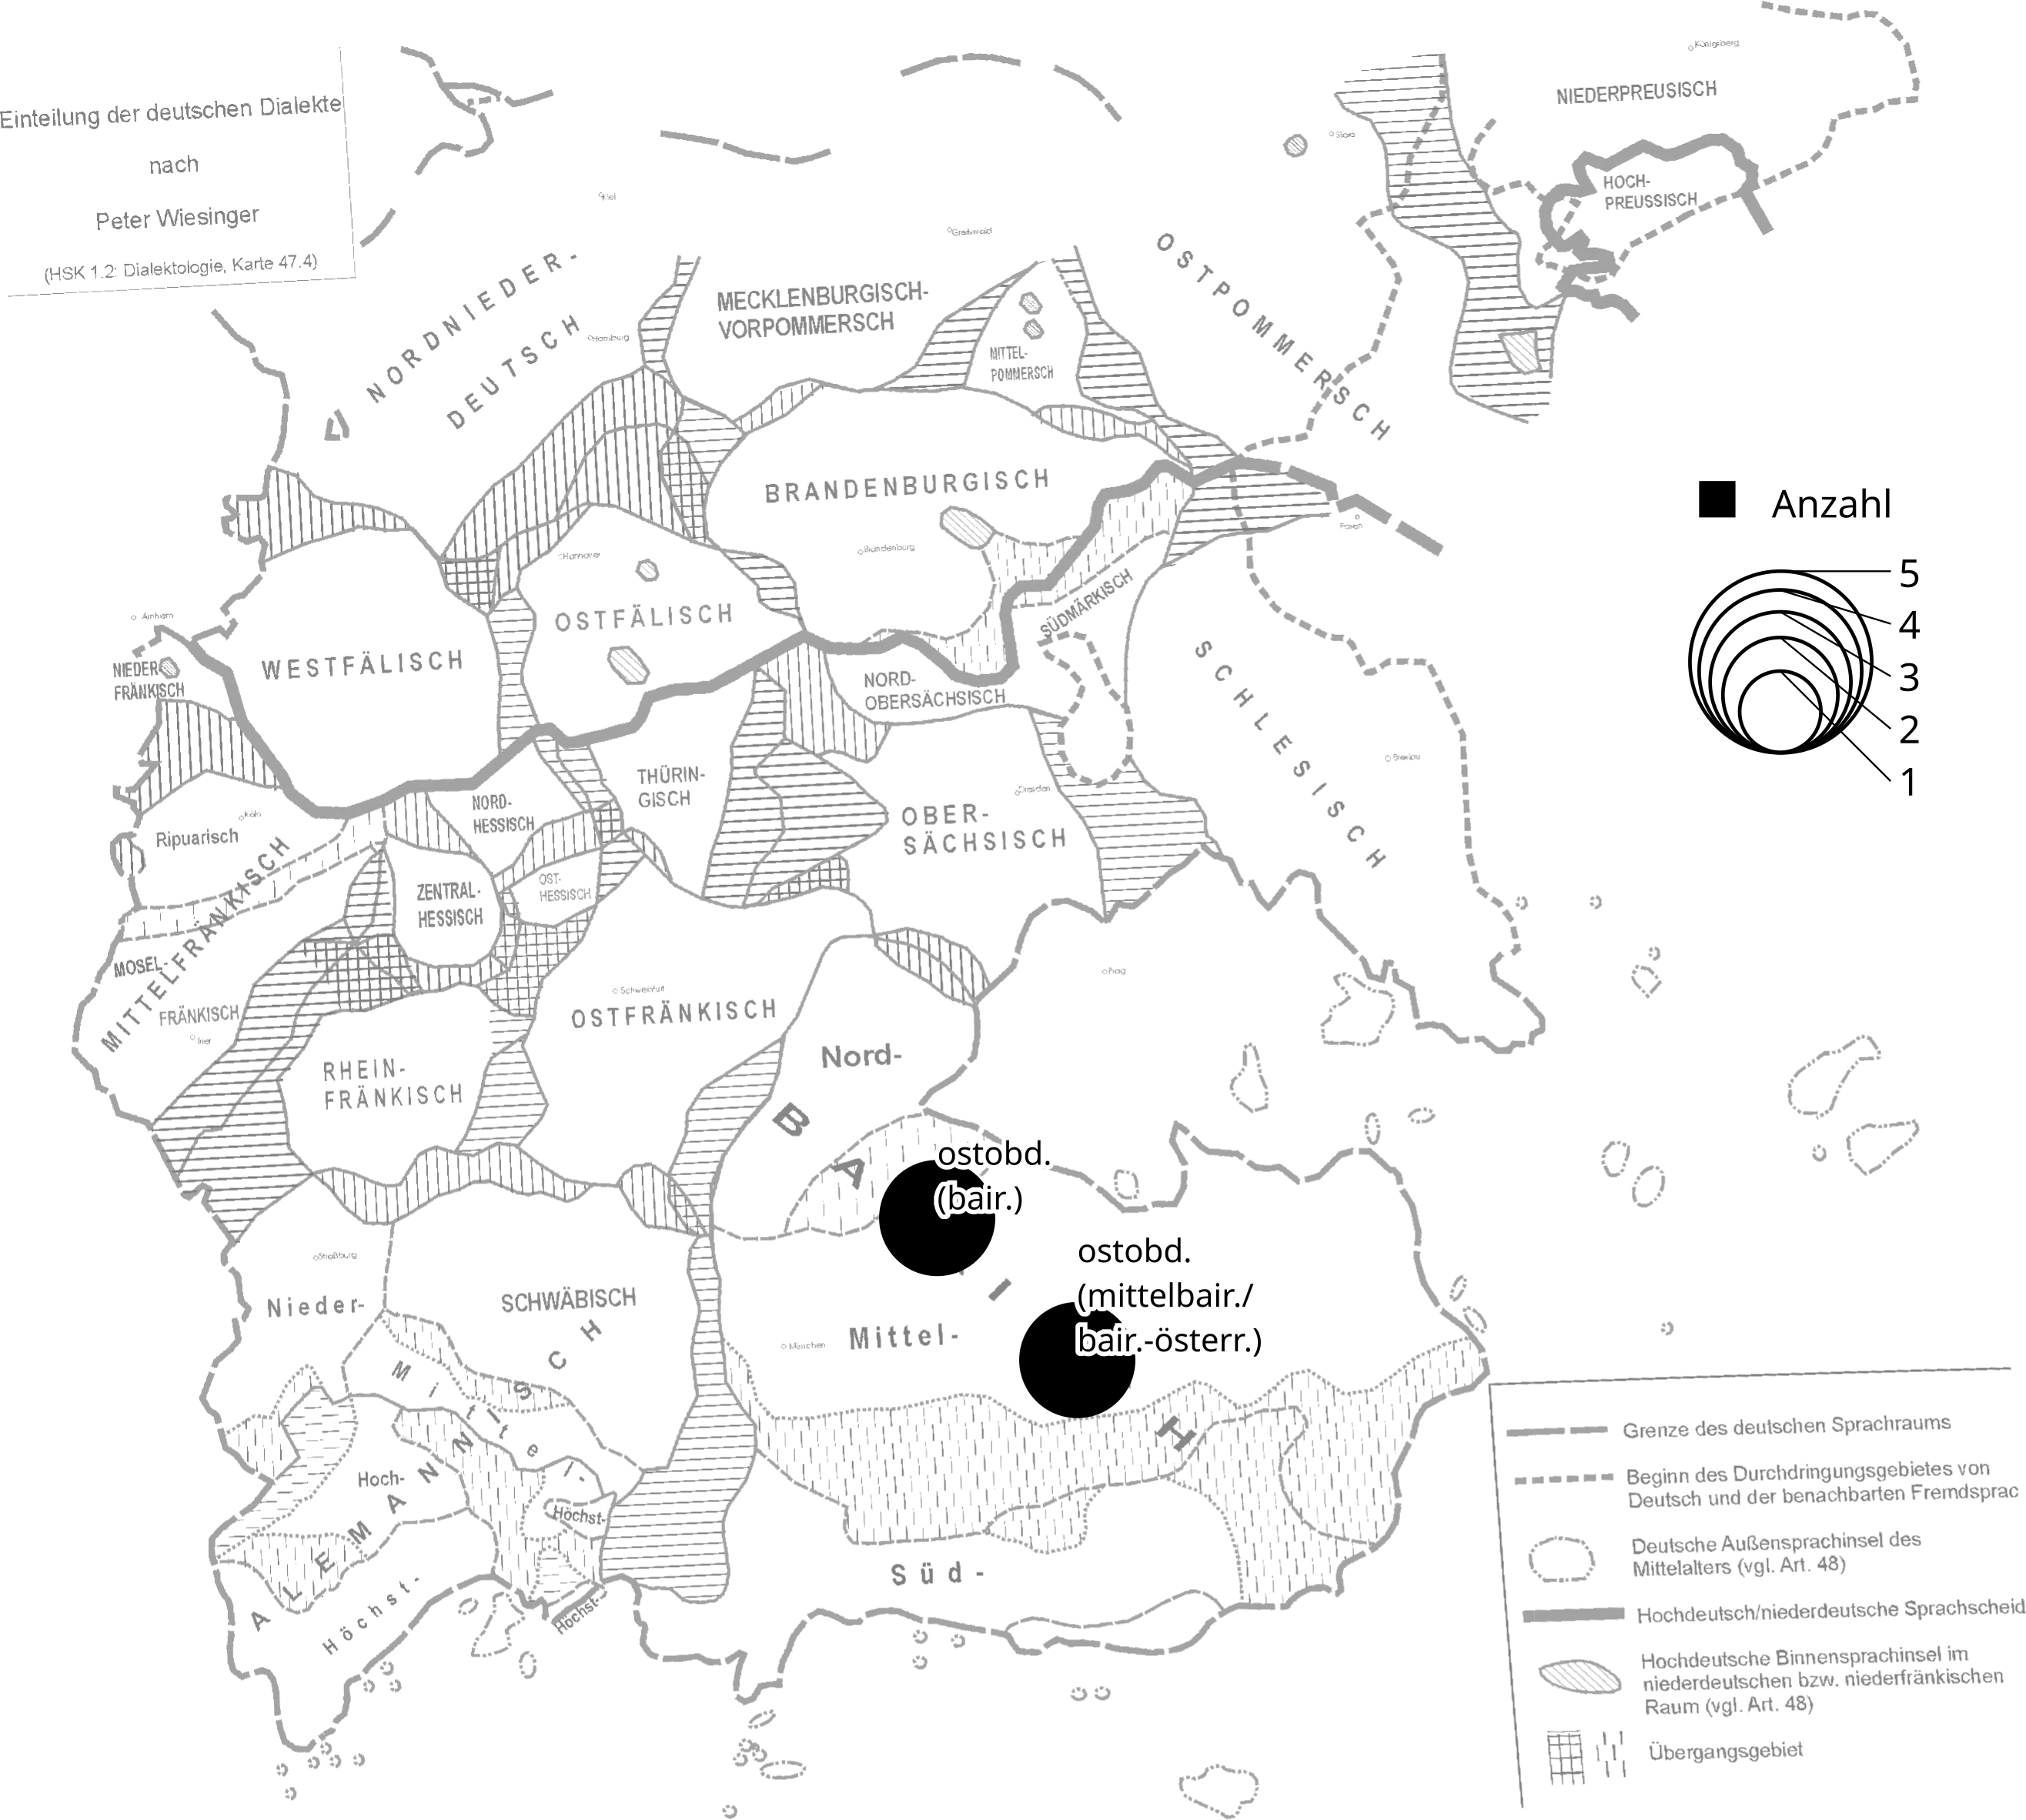
\includegraphics[
	width=\linewidth,
	keepaspectratio
]{./figures/2021-12-30_kc_geospac_rough_c12.png}
\caption%
	{Grobe räumliche und zeitliche Verteilung der \KC{}-Text\-zeugen (12.~Jh.;
	Hintergrundkarte: \cite{wiesinger1983:rede}) }
\label{fig:kc_geospac_rough_12}
\end{figure}

\begin{figure}
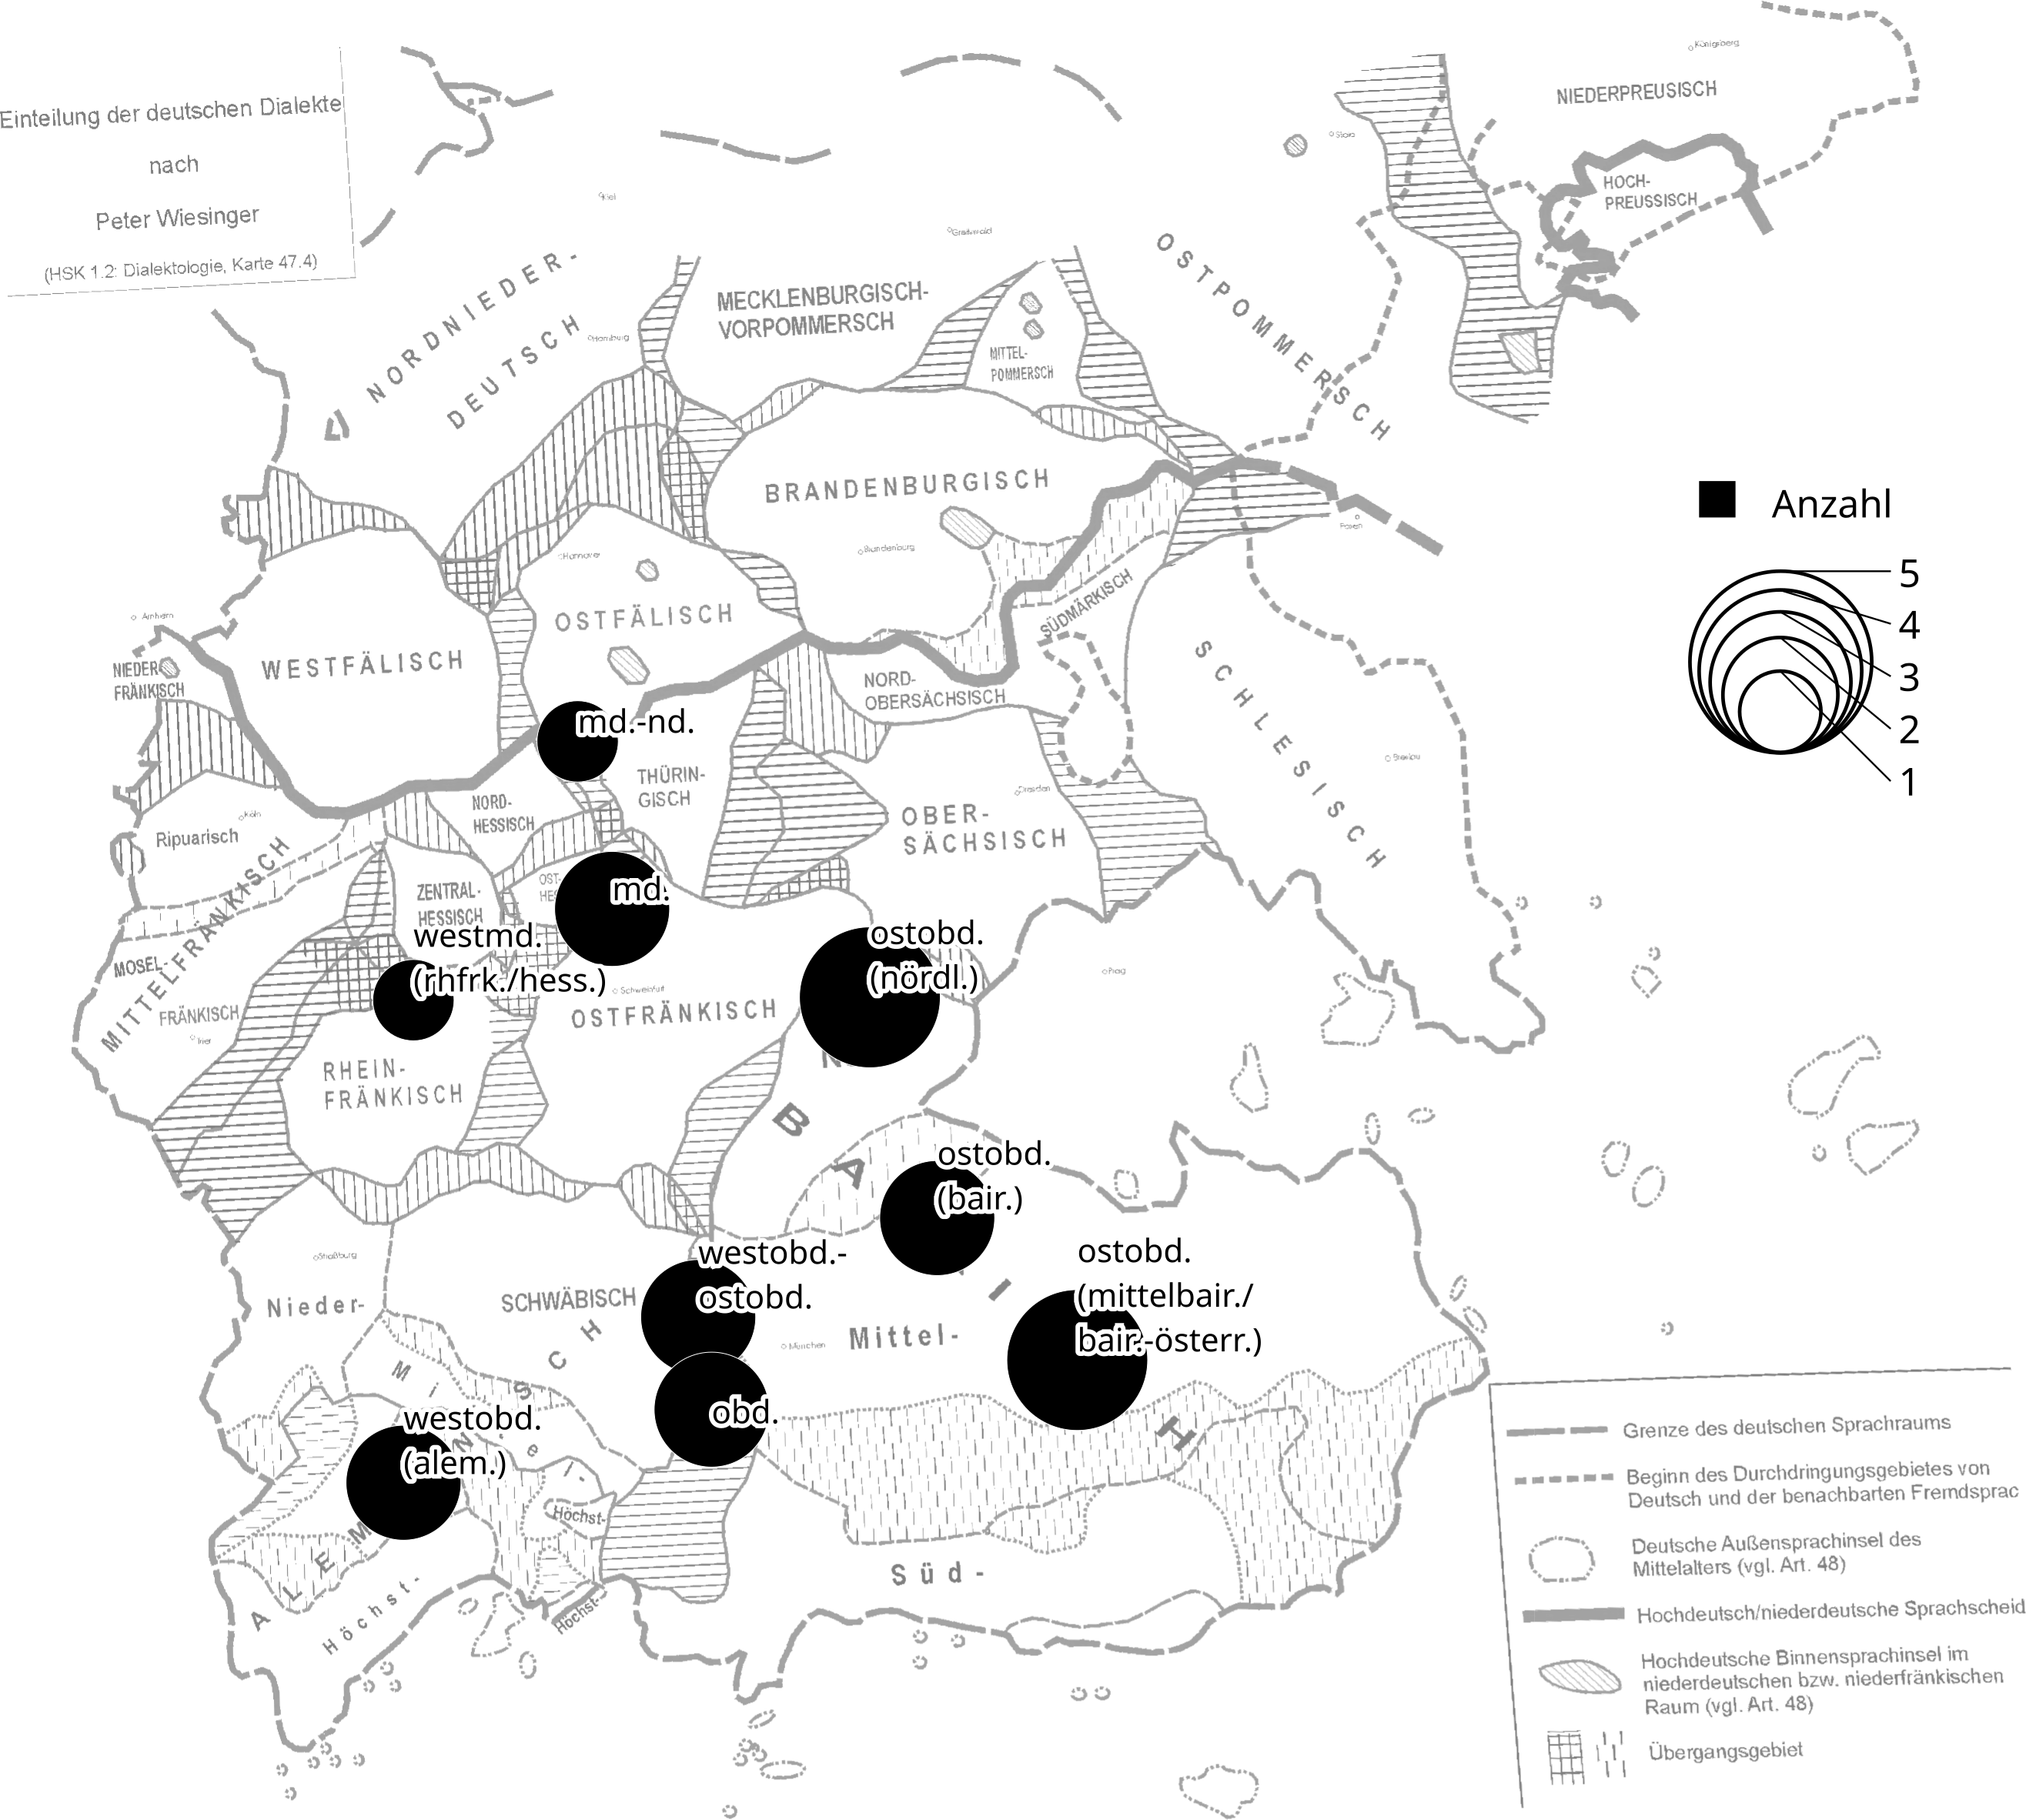
\includegraphics[
	width=\linewidth,
	keepaspectratio
]{./figures/2021-12-30_kc_geospac_rough_c13.png}
\caption%
	{Grobe räumliche und zeitliche Verteilung der \KC{}-Text\-zeugen (13.~Jh.;
	Hintergrundkarte: \cite{wiesinger1983:rede})}
\label{fig:kc_geospac_rough_13}
\end{figure}

\begin{figure}
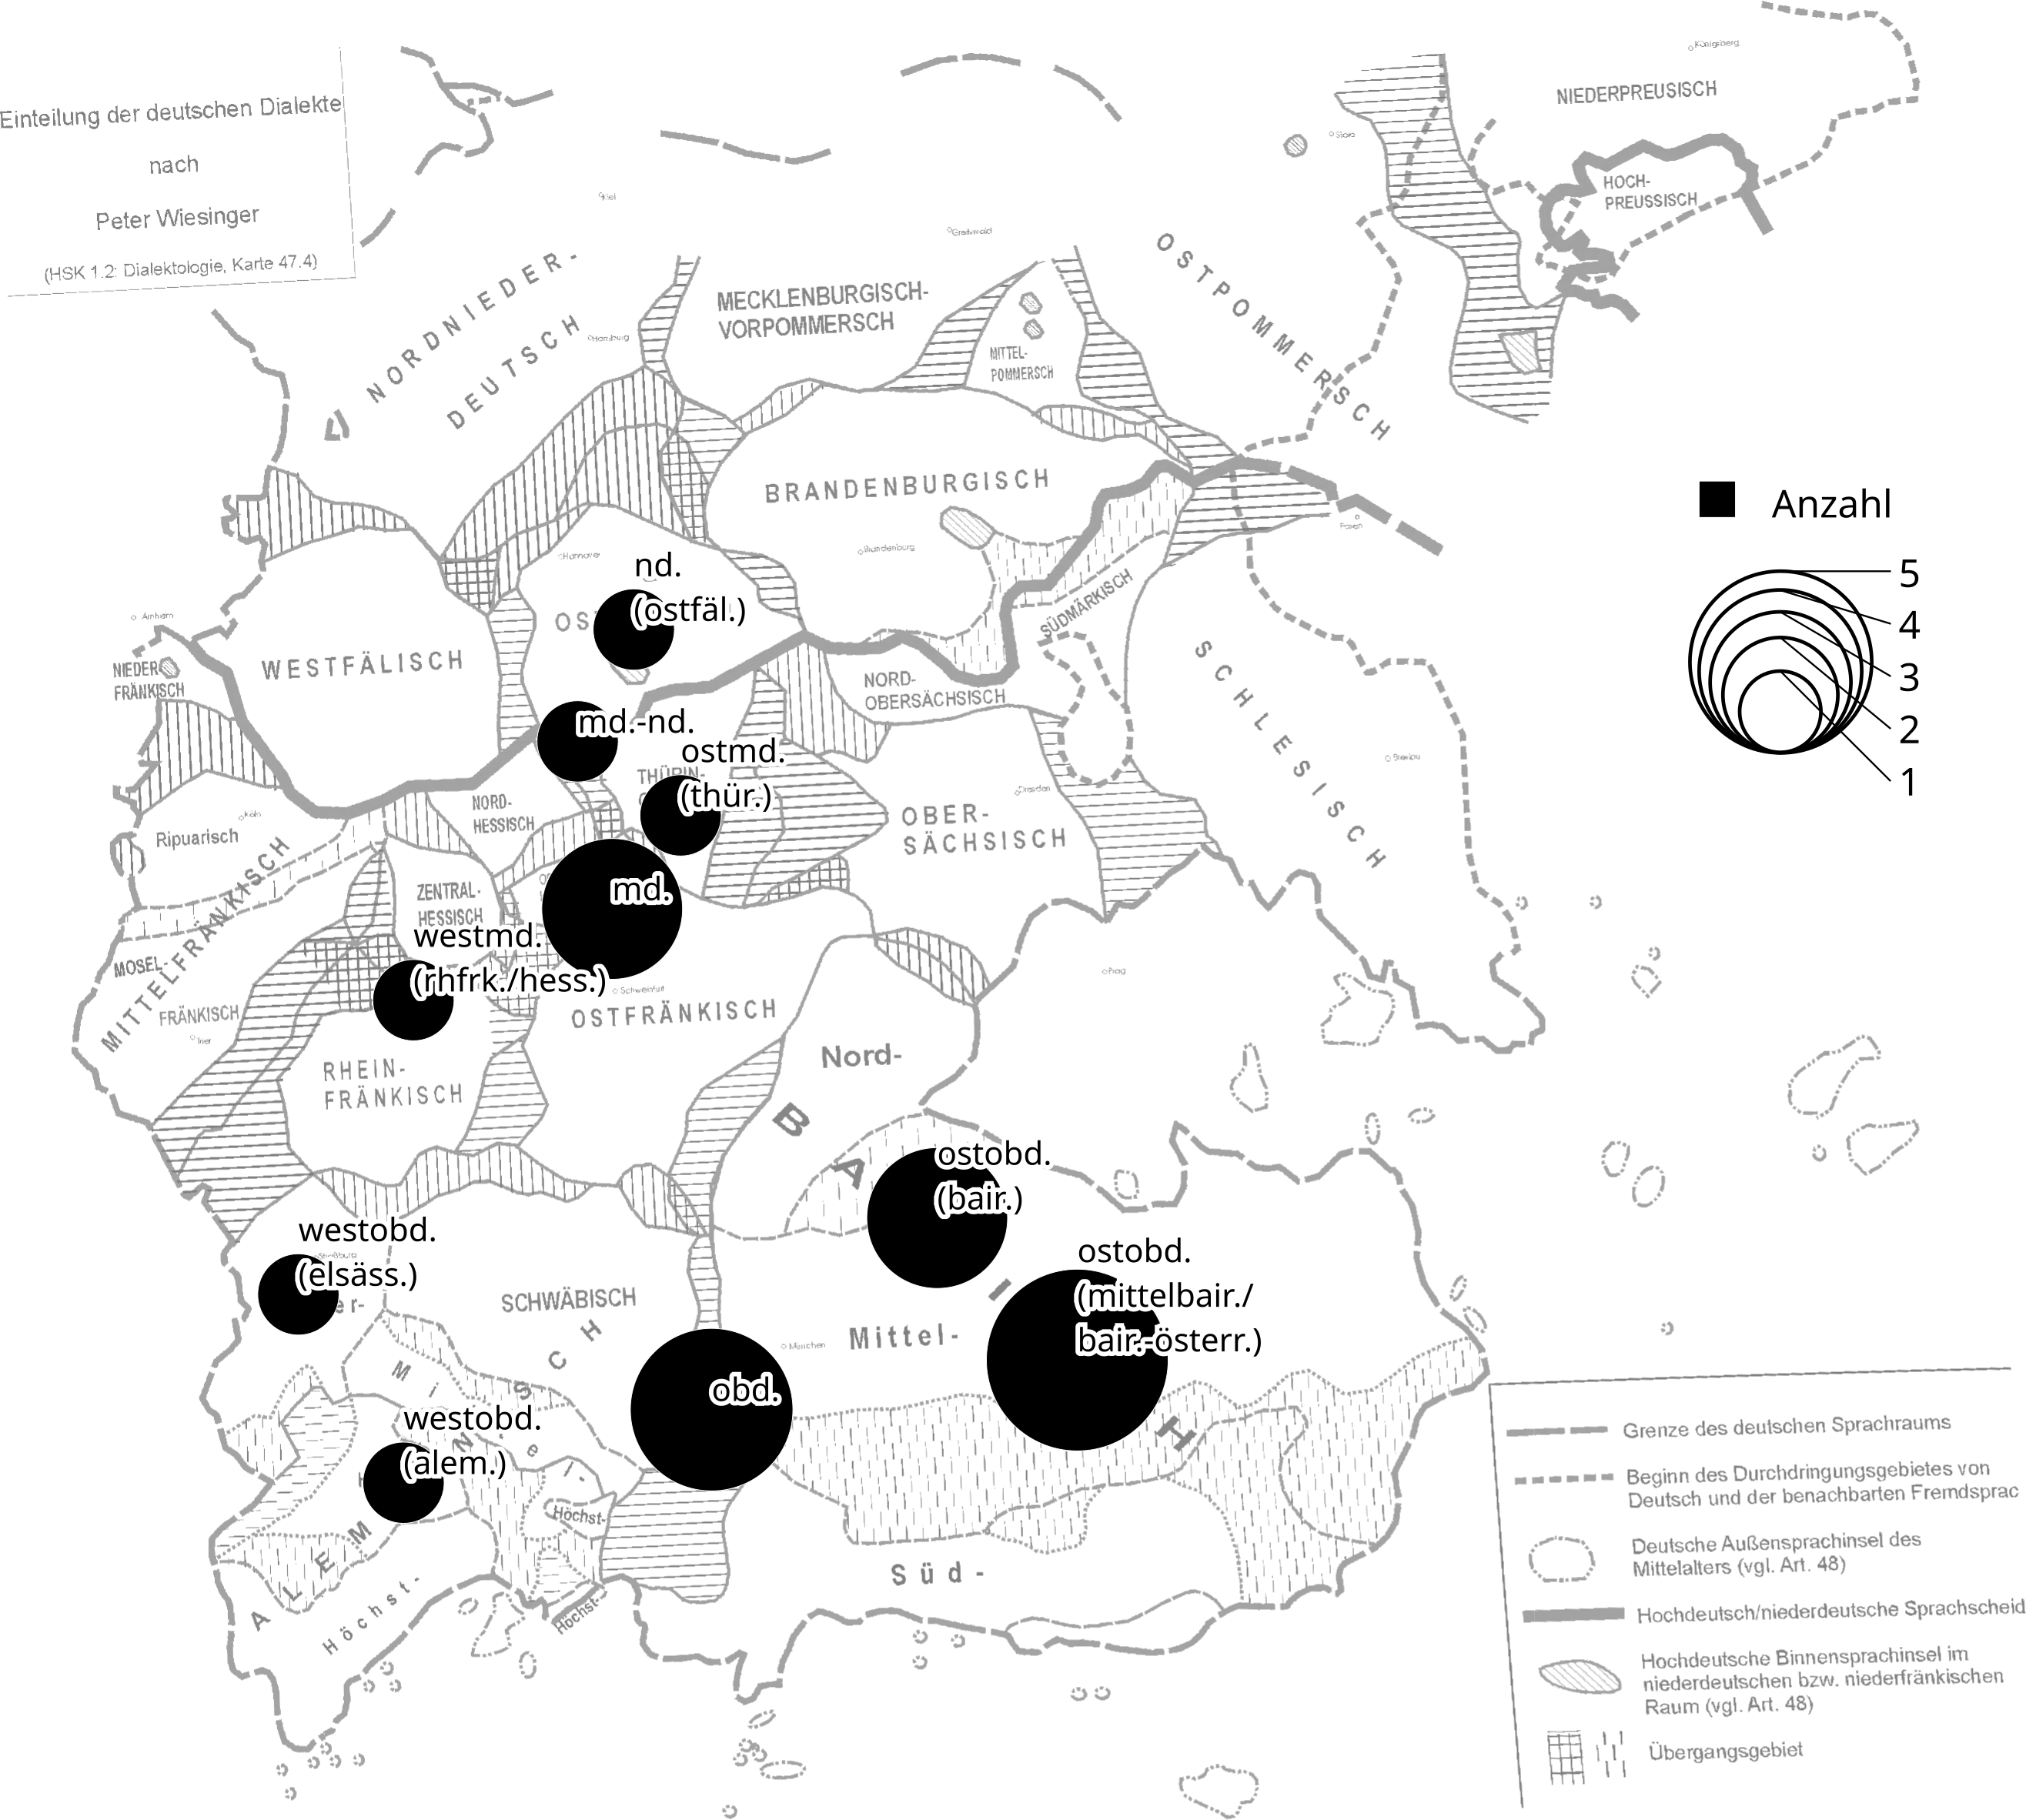
\includegraphics[
	width=\linewidth,
	keepaspectratio
]{./figures/2021-12-30_kc_geospac_rough_c14.png}
\caption%
	{Grobe räumliche und zeitliche Verteilung der \KC{}-Text\-zeugen (14.~Jh.;
	Hintergrundkarte: \cite{wiesinger1983:rede})}
\label{fig:kc_geospac_rough_14}
\end{figure}

\begin{figure}
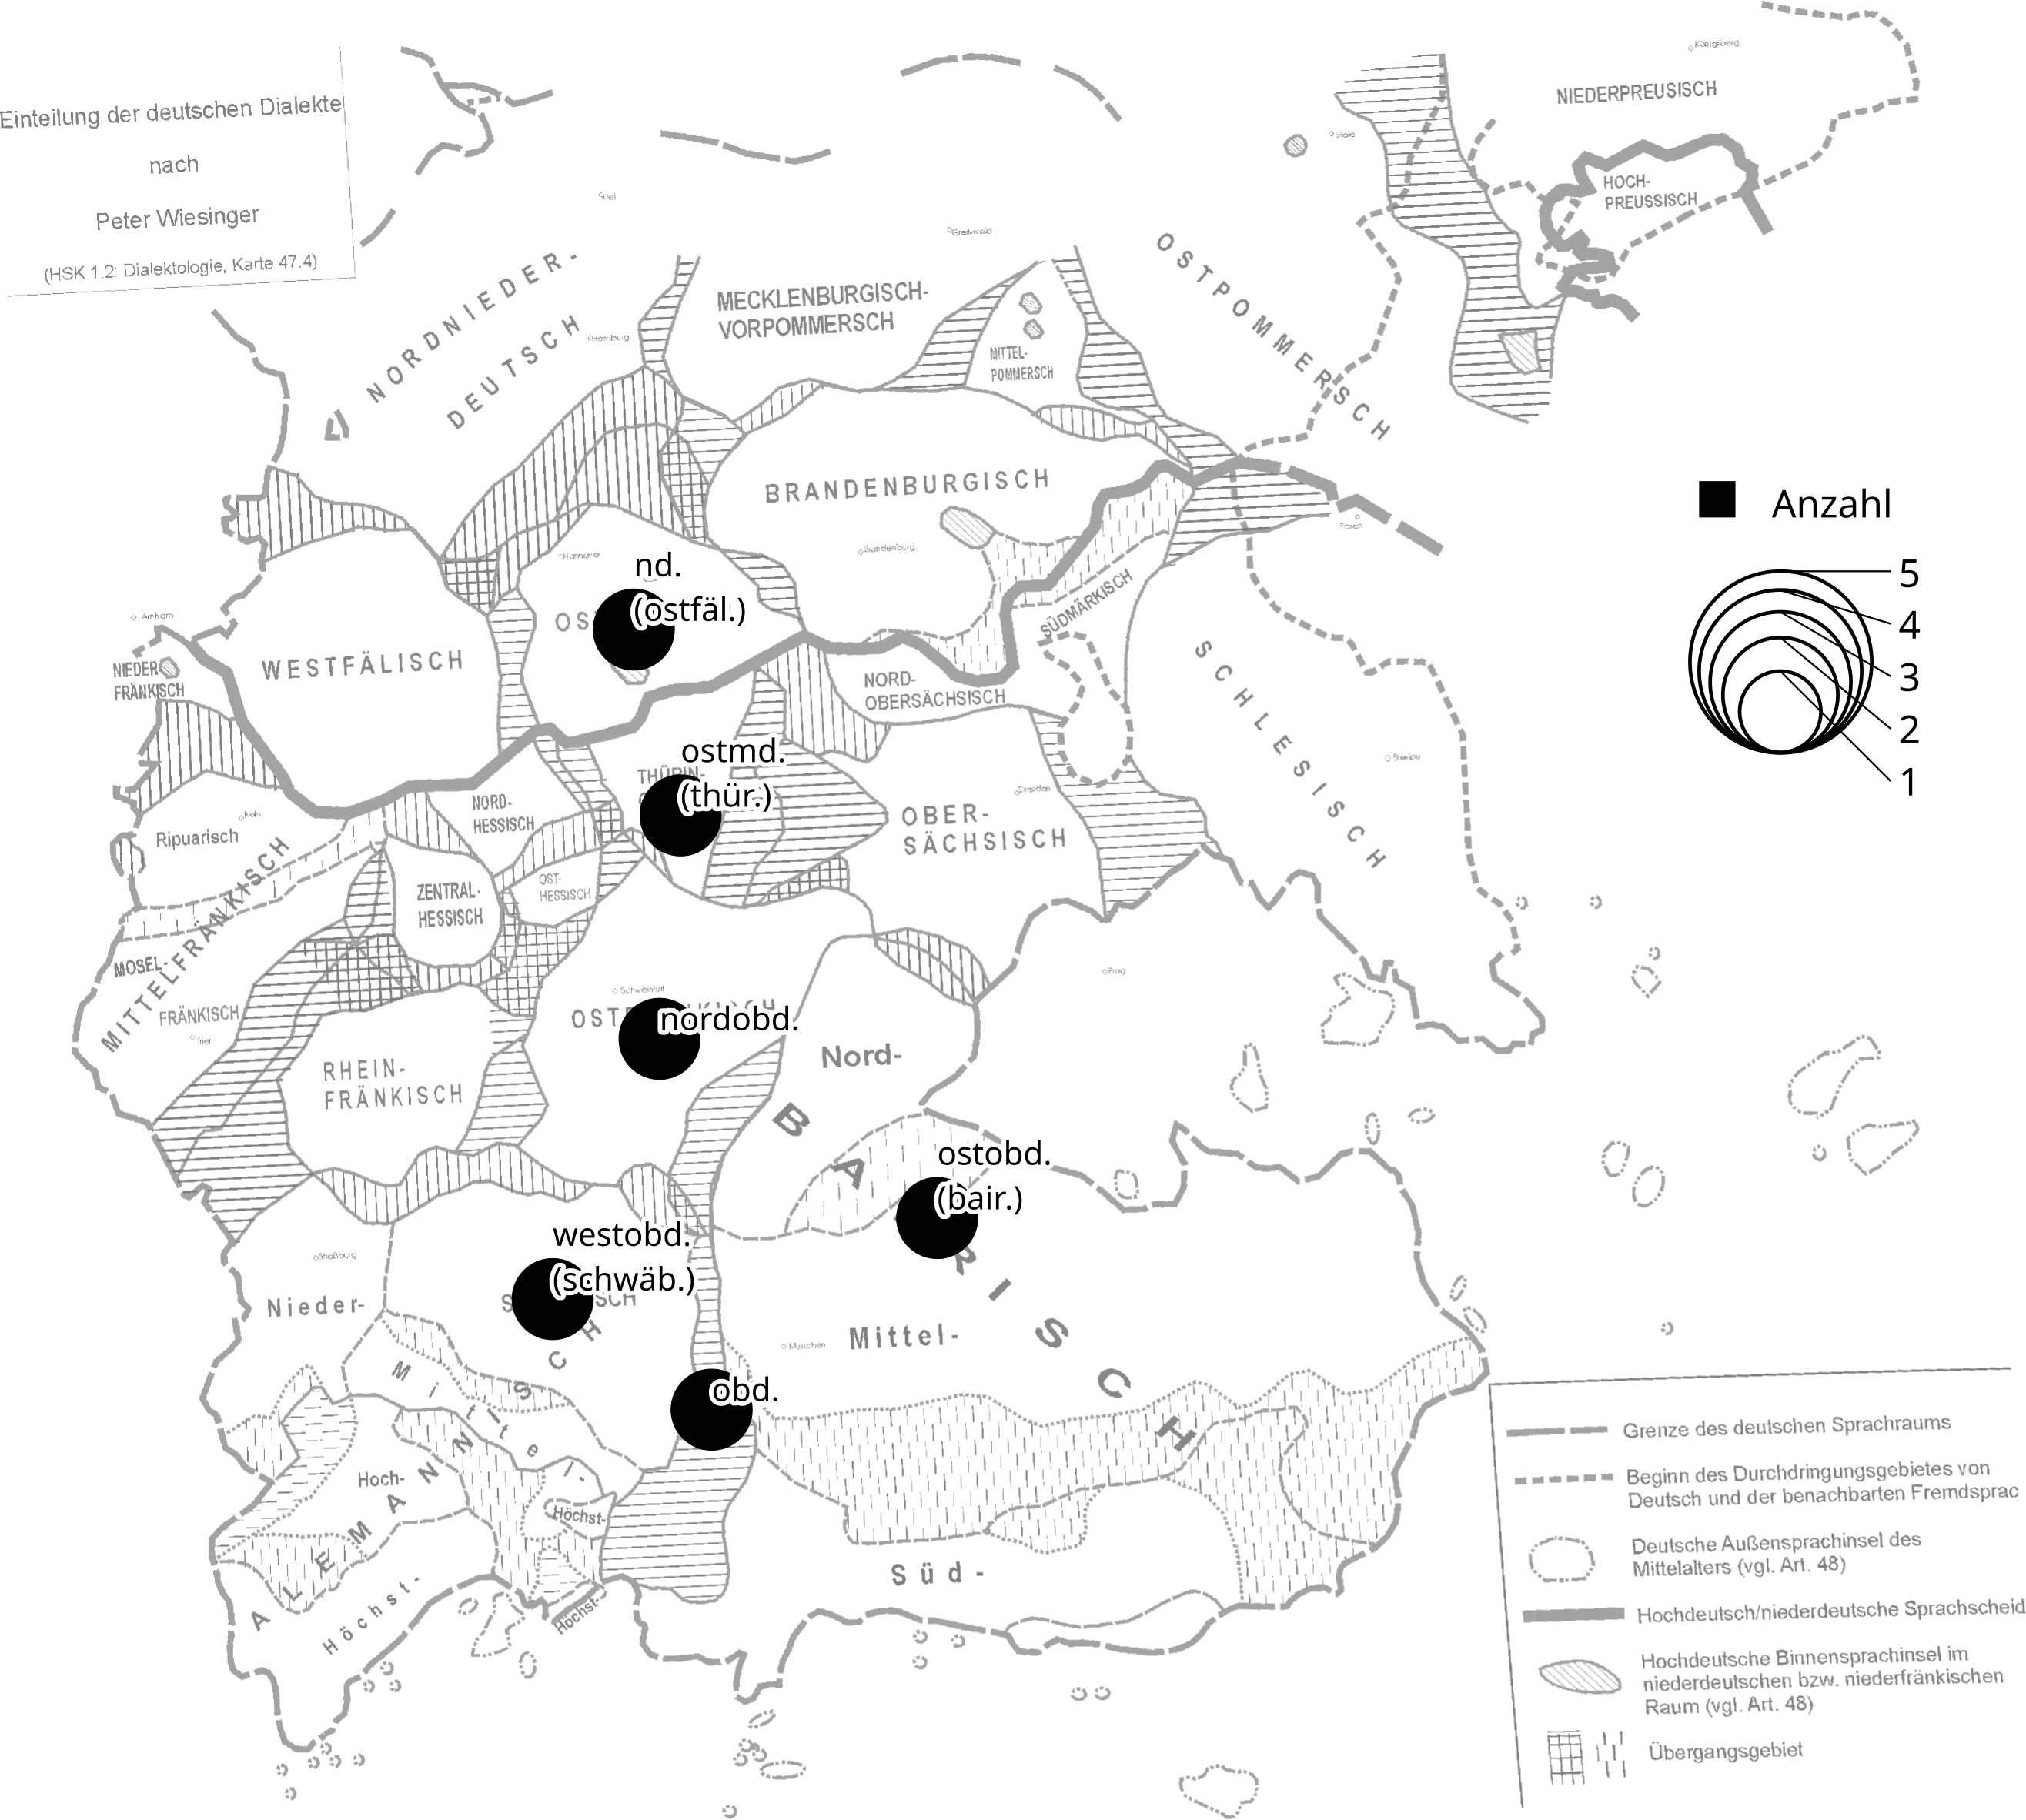
\includegraphics[
	width=\linewidth,
	keepaspectratio
]{./figures/2021-12-30_kc_geospac_rough_c15.png}
\caption%
	{Grobe räumliche und zeitliche Verteilung der \KC{}-Text\-zeugen (15.~Jh.;
	Hintergrundkarte: \cite{wiesinger1983:rede})}
\label{fig:kc_geospac_rough_15}
\end{figure}

Die handschriftliche \isi{Überlieferung} der \KC{} bietet daher ein
entscheidendes Merkmal der geschäftsmäßigen \isi{Schriftlichkeit}
(Urkunden\is{Urkunde}, Urbare) oftmals gerade nicht:
Autornähe\is{Vorlagenproblematik}. Des Weiteren sind die Handschriften der
\KC{} im Gegensatz zu den Urkunden des \CAO{} weder exakt datiert noch
einigermaßen genau lokalisierbar. Aufgrund der von \citet[1310]{wegera2000}
angesprochenen \q{Vorlagenproblematik} muss außerdem davon ausgegangen werden,
dass Dialekt\-mischungen eher die Regel als die Ausnahme darstellen. Der
Vergleich der Daten aus der Auswertung der \KC{} mit denen der
\CAO{}-Auswertung verspricht also besonders valide Ergebnisse, insofern sich
mit Hilfe der Urkunden regionale Merkmale von
Schreibdialekten\is{Schreibdialekt} verorten lassen, trotz der grundsätzlichen
Schreiberproblematik und der Einschränkung, dass die Urkunden lediglich eine
Momentaufnahme der geschriebenen Geschäftssprache des späten 13.~Jahrhunderts
darstellen.

Bezüglich der regionalen Variation von Schreibdialekten\is{Schreibdialekt}
weist \citet{solms2014} darauf hin, \blockcquote[132]{solms2014}{dass es die
überaus große Zersplitterung des Sprachgebietes, wie sie die
Dialektgeographie\is{Dialektgeografie} des 19.~Jahrhunderts erwiesen hat, in
der Schreibsprachlichkeit des 11.\ bis 14.~Jahrhunderts noch nicht gegeben
hat}. Andererseits lässt sich fragen, inwiefern die angesprochene
Zersplitterung ein Artefakt der Erhebungsmethode etwa von Sprachatlanten
darstellt. Dialektgeografische Karten bilden nie die Gesamtheit der
Sprecherinnen und Sprecher mit sämtlichen Variations\-ebenen ab, sondern
unterliegen notwendigerweise Abstraktionen und Vereinfachungen, auch durch die
Auswahl der Informantinnen und Informanten. Diese \isi{Komplexitätsreduktion}
produziert unter Umständen scharfe Grenzen, wo Übergänge in der Realität
fließend sind.
